% !TeX encoding = UTF-8
% !TeX spellcheck = es_AR
% arara: pdflatex
% arara: pdflatex
% arara: pdflatex
% arara: clean: {files: [02_markdown.aux, 02_markdown.out, 02_markdown.log]}
% arara: clean: {files: [02_markdown.fdb_latexmk, 02_markdown.fls, 02_markdown.vrb, 02_markdown.synctex.gz]}

%% Add the word "answers" to document class parameters in order to print the solutions.
\documentclass[12pt, addpoints]{../../common/epyl_exam_template}

\title{Práctica 1.2 - Markdown}
\date{2018.1}

\begin{document}
\makeexamheader
\makeexamtitle
\examrule

\begin{questions}
  \question
    Dado el siguiente texto en Markdown, resaltar en negrita los sujetos, y
    en cursiva los verbos.
    \begin{quoted}
      La ley de Moore expresa lo siguiente:
      El numero de transistores en un microprocesador se duplica aproximadamente
      cada dos años.

      La consecuencia directa de la ley de Moore será que los precios bajan al
      mismo tiempo que las prestaciones suben. Así, la computadora que hoy
      vale 3000 dólares costará la mitad al año siguiente y estará obsoleta en
      dos años. En 26 años el número de transistores en un chip se
      incrementó 3200 veces.
    \end{quoted}

    \begin{solution}
      \begin{lstlisting}[language=Markdown]
**La ley de Moore** _expresa_ lo siguiente: (*\Suppressnumber*)
**El numero de transistores en un microprocesador**
_se_ duplica aproximadamente cada dos años. (*\Reactivatenumber*)

**La consecuencia directa de la ley de Moore** _será_ (*\Suppressnumber*)
que los precios bajan al mismo tiempo que las prestaciones
suben. Así, **la computadora que hoy vale 3000 dólares**
_costará_ la mitad al año siguiente y _estará_ obsoleta
en dos años. En 26 años **el número de transistores
en un chip** _incrementó_ 3200 veces. (*\Reactivatenumber*)
      \end{lstlisting}
    \end{solution}

  \question
    Buscar en internet la receta para hacer tallarines caseros, y redactarla
    prolijamente en Markdown. Utilizar una lista no ordenada para los
    ingredientes, y una lista ordenada para los pasos a seguir.

    \begin{solution}
      \begin{lstlisting}[language=Markdown]
Tallarines al huevo
===================

Ingredientes
------------
* Harina com\'un (900gr)
* Huevos (6 unidades)
* Vinagre (50cc)
* Aceite (50cc)
* Agua (cantidad necesaria)
* Sal (a gusto)

Pasos a seguir
--------------

1. Poner la harina en la mesada, hacer un hueco (*\Suppressnumber*)
  y colocar en el mismo huevos, vinagre y aceite (*\Reactivatenumber*)
2. Unimos un poco y vamos agregando el agua (*\Suppressnumber*)
  hasta unir y formar una masa dura. (*\Reactivatenumber*)
3. Estirarla fina. Dejar reposar por 10 minutos.
4. Cortar los tallarines realizando tiras pequeñas.
5. Hervir en abundante agua y servir acompañada de (*\Suppressnumber*)
  alguna salsa.(*\Reactivatenumber*)
      \end{lstlisting}
    \end{solution}

  \question
    Buscar las imágenes de los 3 lugares del mundo que más desearías
    visitar. Insertar las imágenes en un documento Markdown, colocando el
    nombre del lugar como titulo de nivel 3 y el país en el que se encuentra
    como subtitulo de nivel 5. Hacer que el título sea un hipervínculo a
    la página de wikipedia sobre ese lugar.

    \begin{solution}
      \begin{lstlisting}[language=Markdown]
### [Santuario Histórico de Machu Picchu](*\Suppressnumber*)
(https://es.wikipedia.org/wiki/Machu_Picchu)(*\Reactivatenumber*)
##### Perú
![Machu Picchu](https://upload.wikimedia.org/wikipedia/commons/(*\Suppressnumber*)
thumb/1/13/Before_Machu_Picchu.jpg/
1024px-Before_Machu_Picchu.jpg)(*\Reactivatenumber*)

### [Pirámides de Egipto](*\Suppressnumber*)
(https://es.wikipedia.org/wiki/Pirámides_de_Egipto)(*\Reactivatenumber*)

##### Egipto
![Pirámides de Giza](https://upload.wikimedia.org/wikipedia/(*\Suppressnumber*)
commons/thumb/a/af/All_Gizah_Pyramids.jpg/
1920px-All_Gizah_Pyramids.jpg)(*\Reactivatenumber*)

### [La Gran Muralla China](*\Suppressnumber*)
(https://es.wikipedia.org/wiki/Gran_Muralla_China)(*\Reactivatenumber*)
##### China
![La Gran Muralla China](https://upload.wikimedia.org/(*\Suppressnumber*)
wikipedia/commons/thumb/2/23/
The_Great_Wall_of_China_at_Jinshanling-edit.jpg/
1920px-The_Great_Wall_of_China_at_Jinshanling-edit.jpg)(*\Reactivatenumber*)
      \end{lstlisting}
    \end{solution}

  \question
    Realizar un dibujo (esquema) en donde se muestre el resultado del
    siguiente código markdown tras ser leído por un visualizador.\\~\\
    \textit{El objetivo es realizar el dibujo previo a visualizarlo, pero
    puede copiar el código en un visualizador para contrastar su respuesta
    con el resultado real}.

    \begin{lstlisting}[language=markdown]
# AFA-NO
## Asociación de Futsal Amateur - No Oficial

----

+ [Sobre el futsal](futsal.html)
+ [Sobre nosotros](nosotros.html)
  - [Quienes somos](somos.html)
  - [Que queremos](somos.html)

----

El futsal es un deporte **apasionante** que involucra
destreza, equilibrio físico y un montón de aguante.

----

Venga a nuestros puntos de encuentro:

1. Cementerio de la Chacarita
2. Campo de Mayo
3. Rotonda de Alpargatas
4. Delta del Tigre

----

Copyright: AFA-NO
    \end{lstlisting}
    \begin{solution}
      \frame{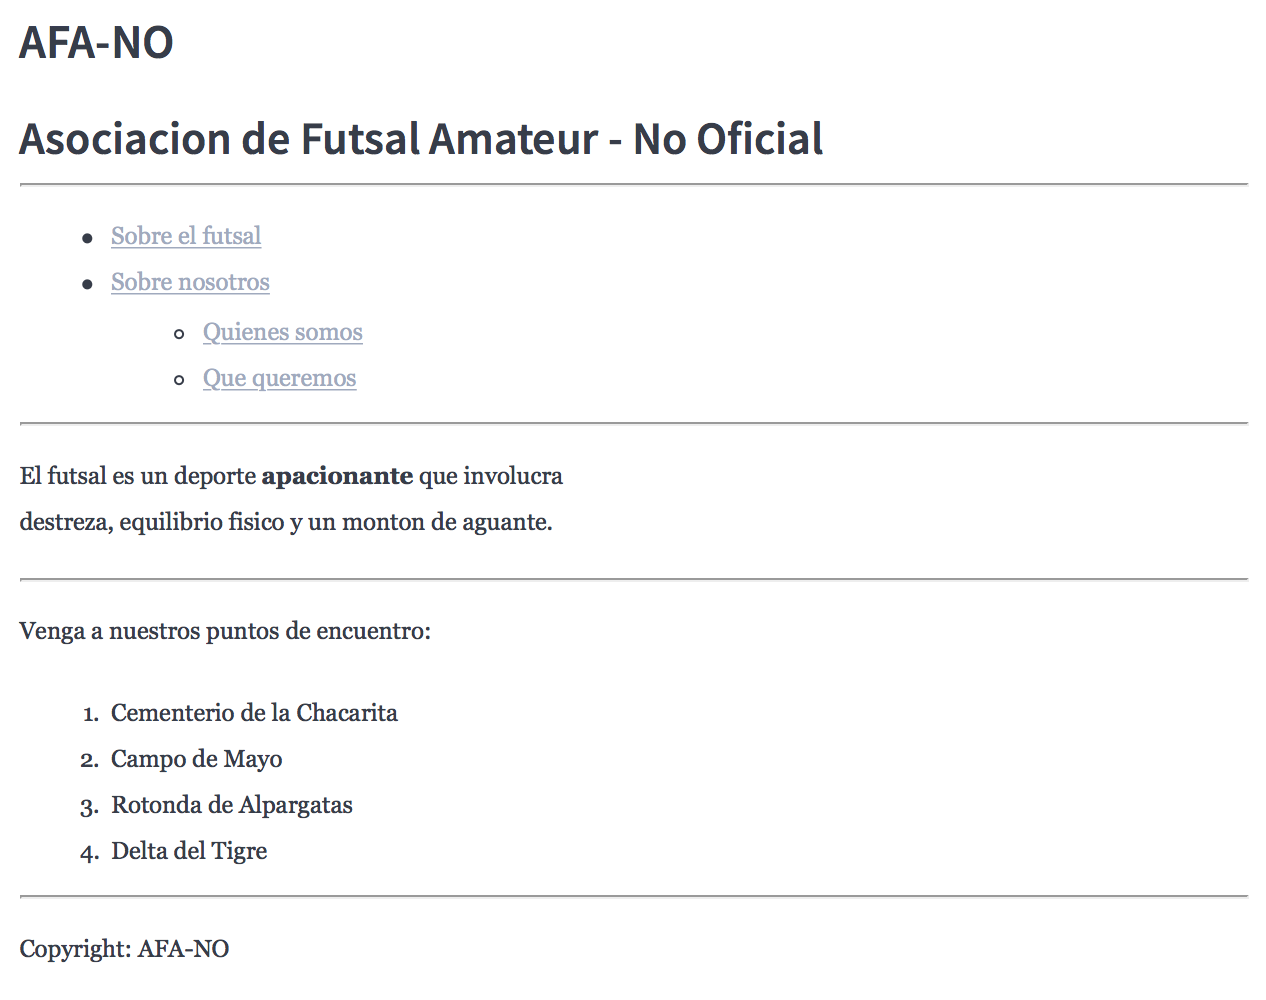
\includegraphics[scale=0.675]{img/afa_no.png}}
    \end{solution}

  \question
    Para este ejercicio deberá utilizar su correo electrónico. Escriba un correo
    al docente de la materia en donde responda a las siguientes secciones:
    \begin{itemize}
      \item Cuál es su nombre y apellido completo. Donde vive (no hace falta
        dirección, barrio y ciudad son suficientes). Si nació en algún otro
        lado y vino al país/provincia/ciudad a estudiar, dónde y hace cuanto
        tiempo se mudó.
      \item ¿Trabaja? Si la respuesta es si, cuente si su trabajo se
        relaciona o no con la carrera que cursa y cuantas horas trabaja en
        general. También si su trabajo le permite flexibilidad horaria para
        asistir a la cursada y si puede o no tomarse días por examen.
        Si no trabaja, nos interesa saber si busca trabajo activamente o si
        no tiene interés de trabajar por el momento.
      \item Cuánto tiempo le lleva arribar a la universidad y en que
        transporte viene. Si viene desde el trabajo, cuéntenos donde está
        ubicado el trabajo y si le resulta difícil llegar a la cursada.
      \item ¿Es la primera vez que cursa esta asignatura? Si no es la primera
        vez, qué motivos cree que lo han hecho desaprobar. Qué estrategias
        planea seguir para aprobar la asignatura en esta oportunidad.
    \end{itemize}
    El correo deberá ser escrito utilizando markdown, seccionando correctamente
    las distintas partes utilizando subtítulos, y tener formato utilizando negritas,
    cursivas y listados donde le resulte conveniente.

  \question
    Elabore su curriculum vitae utilizando markdown. Para ello, coloque su nombre
    completo como título, agregue una foto de su persona, y seccione el contenido
    correctamente utilizando títulos y subtítulos. Liste los trabajos y formación
    con la que cuenta. No hace falta que el CV sea verdadero, basta con que sea
    verosímil.

\end{questions}
\end{document}
